\begin{frame}{はじめに}

Rマークダウンでドキュメントとコード書いて→ knit() → pandoc → (html
\textbar{} pdf \textbar{} docx) します。

\begin{block}{役に立つ資料}

\begin{itemize}
\itemsep1pt\parskip0pt\parsep0pt
\item
  @teramonagiさんの資料

  \begin{itemize}
  \itemsep1pt\parskip0pt\parsep0pt
  \item
    Tokyo.R@36 ~knitr+pandocではじめる~『R MarkdownでReproducible
    Research』
    \url{http://www.slideshare.net/teramonagi/tokyo-r36-20140222}
  \item
    Tokyo.R@36 ~knitrパッケージではじめる~『R MarkdownでReproducible
    Research』の基礎編のコード
    \url{http://rpubs.com/teramonagi/TokyoR36_Basic}
  \item
    Tokyo.R@36 ~knitrパッケージではじめる~『R MarkdownでReproducible
    Research』の応用編のコード
    \url{http://rpubs.com/teramonagi/TokyoR36_Advanced}
  \end{itemize}
\item
  Pandoc ユーザーズガイド 日本語版
  \url{http://sky-y.github.io/site-pandoc-jp/users-guide/}
\item
  TeX Wiki \url{http://oku.edu.mie-u.ac.jp/~okumura/texwiki/}
\item
  マークダウン用 github.css
  \url{https://gist.github.com/andyferra/2554919}
\end{itemize}

も参考にしてくださいね〜

\end{block}

\end{frame}

\begin{frame}[fragile]{メタ情報の記述}

マークダウンファイルにはメタ情報を含めることができます。

\begin{block}{簡易記法}

ファイル先頭を

\begin{verbatim}
% タイトル
% 著者
% 日付
\end{verbatim}

で始めることができます。

\end{block}

\begin{block}{YAML記法}

ファイルの先頭にYAMLでメタ情報を入れることができます。次の例を参考にして下さい。

\begin{verbatim}
---
title: RマークダウンとPandocで楽々レポート作成
author: "@ohske"
tags: [R, pandoc, Dynamic Documentation]
abstract: Rマークダウンでドキュメントとコード書いて→ knit() → pandoc → (html | pdf | docx)します。
---
\end{verbatim}

\end{block}

\end{frame}

\begin{frame}[fragile]{レポート生成コマンド (おなじない)}

まずは、

\begin{Shaded}
\begin{Highlighting}[]
\KeywordTok{library}\NormalTok{(knitr)}
\KeywordTok{knit}\NormalTok{(}\StringTok{"pandoc-md.Rmd"}\NormalTok{)}
\end{Highlighting}
\end{Shaded}

としてRマークダウンファイル(.Rmd)からマークダウンファイルを作成します。
続いて、マークダウンファイルをPandocによって様々な形式に変換します。

\begin{itemize}
\item
  HTMLファイルの作成

\begin{Shaded}
\begin{Highlighting}[]
\NormalTok{$ }\KeywordTok{pandoc} \NormalTok{-s --toc -c github.css --mathjax pandoc-md.md -o pandoc-md.html}
\end{Highlighting}
\end{Shaded}

  github.cssというファイルを同じフォルダに入れときます。
\item
  LaTeXファイルの作成

\begin{Shaded}
\begin{Highlighting}[]
\NormalTok{$ }\KeywordTok{pandoc} \NormalTok{-s --toc --number-sections -V documentclass=ltjarticle pandoc-md.md -o pandoc-md.tex}
\end{Highlighting}
\end{Shaded}
\item
  PDFファイルの作成

\begin{Shaded}
\begin{Highlighting}[]
\NormalTok{$ }\KeywordTok{pandoc} \NormalTok{-s --toc --number-sections --listings -V documentclass=ltjarticle --latex-engine=lualatex pandoc-md.md -o pandoc-md.pdf}
\end{Highlighting}
\end{Shaded}
\item
  DOCXファイルの作成

\begin{Shaded}
\begin{Highlighting}[]
\NormalTok{$ }\KeywordTok{pandoc} \NormalTok{-s pandoc-md.md -o pandoc-md.docx}
\end{Highlighting}
\end{Shaded}
\end{itemize}

\begin{block}{R上でpandocを使う}

knitrパッケージには\texttt{pandoc()}という関数があるんですが、オプション渡すのが面倒なので\texttt{system()}でpandocを実行します。

\begin{Shaded}
\begin{Highlighting}[]
\KeywordTok{system}\NormalTok{(}\StringTok{"pandoc -s --toc -c github.css --mathjax pandoc-md.md -o pandoc-md.html"}\NormalTok{)}
\KeywordTok{system}\NormalTok{(}\StringTok{"pandoc -s --toc --number-sections -V documentclass=ltjarticle pandoc-md.md -o pandoc-md.tex"}\NormalTok{)}
\KeywordTok{system}\NormalTok{(}\StringTok{"pandoc -s --toc --number-sections --listings -V documentclass=ltjarticle --latex-engine=lualatex pandoc-md.md -o pandoc-md.pdf"}\NormalTok{)}
\KeywordTok{system}\NormalTok{(}\StringTok{"pandoc -s pandoc-md.md -o pandoc-md.docx"}\NormalTok{)}
\end{Highlighting}
\end{Shaded}

\end{block}

\end{frame}

\begin{frame}[fragile]{例:あやめの解析 (またかよ・・・orz)}

\textbf{あやめ}とは、\sout{さかな}植物の名前です。おそらく、世界中でも最も多く解析にさらされた植物でしょう。

学名は\emph{Iris sanguinea}といいます。イリスではなくて、アイリスです。
\textsubscript{大きい声では言えませんが今でも「イリス」と呼んでます。}

\begin{block}{データの雰囲気}

\begin{Shaded}
\begin{Highlighting}[]
\NormalTok{pander::}\KeywordTok{pandoc}\NormalTok{(}\KeywordTok{head}\NormalTok{(iris), }\DataTypeTok{caption=}\StringTok{"あやめのデータ (1-6行)"}\NormalTok{, }\DataTypeTok{split.tables =} \DecValTok{100}\NormalTok{)}
\end{Highlighting}
\end{Shaded}

\begin{longtable}[c]{@{}ccccc@{}}
\toprule\addlinespace
\begin{minipage}[b]{0.18\columnwidth}\centering
Sepal.Length
\end{minipage} & \begin{minipage}[b]{0.17\columnwidth}\centering
Sepal.Width
\end{minipage} & \begin{minipage}[b]{0.18\columnwidth}\centering
Petal.Length
\end{minipage} & \begin{minipage}[b]{0.17\columnwidth}\centering
Petal.Width
\end{minipage} & \begin{minipage}[b]{0.11\columnwidth}\centering
Species
\end{minipage}
\\\addlinespace
\midrule\endhead
\begin{minipage}[t]{0.18\columnwidth}\centering
5.1
\end{minipage} & \begin{minipage}[t]{0.17\columnwidth}\centering
3.5
\end{minipage} & \begin{minipage}[t]{0.18\columnwidth}\centering
1.4
\end{minipage} & \begin{minipage}[t]{0.17\columnwidth}\centering
0.2
\end{minipage} & \begin{minipage}[t]{0.11\columnwidth}\centering
setosa
\end{minipage}
\\\addlinespace
\begin{minipage}[t]{0.18\columnwidth}\centering
4.9
\end{minipage} & \begin{minipage}[t]{0.17\columnwidth}\centering
3
\end{minipage} & \begin{minipage}[t]{0.18\columnwidth}\centering
1.4
\end{minipage} & \begin{minipage}[t]{0.17\columnwidth}\centering
0.2
\end{minipage} & \begin{minipage}[t]{0.11\columnwidth}\centering
setosa
\end{minipage}
\\\addlinespace
\begin{minipage}[t]{0.18\columnwidth}\centering
4.7
\end{minipage} & \begin{minipage}[t]{0.17\columnwidth}\centering
3.2
\end{minipage} & \begin{minipage}[t]{0.18\columnwidth}\centering
1.3
\end{minipage} & \begin{minipage}[t]{0.17\columnwidth}\centering
0.2
\end{minipage} & \begin{minipage}[t]{0.11\columnwidth}\centering
setosa
\end{minipage}
\\\addlinespace
\begin{minipage}[t]{0.18\columnwidth}\centering
4.6
\end{minipage} & \begin{minipage}[t]{0.17\columnwidth}\centering
3.1
\end{minipage} & \begin{minipage}[t]{0.18\columnwidth}\centering
1.5
\end{minipage} & \begin{minipage}[t]{0.17\columnwidth}\centering
0.2
\end{minipage} & \begin{minipage}[t]{0.11\columnwidth}\centering
setosa
\end{minipage}
\\\addlinespace
\begin{minipage}[t]{0.18\columnwidth}\centering
5
\end{minipage} & \begin{minipage}[t]{0.17\columnwidth}\centering
3.6
\end{minipage} & \begin{minipage}[t]{0.18\columnwidth}\centering
1.4
\end{minipage} & \begin{minipage}[t]{0.17\columnwidth}\centering
0.2
\end{minipage} & \begin{minipage}[t]{0.11\columnwidth}\centering
setosa
\end{minipage}
\\\addlinespace
\begin{minipage}[t]{0.18\columnwidth}\centering
5.4
\end{minipage} & \begin{minipage}[t]{0.17\columnwidth}\centering
3.9
\end{minipage} & \begin{minipage}[t]{0.18\columnwidth}\centering
1.7
\end{minipage} & \begin{minipage}[t]{0.17\columnwidth}\centering
0.4
\end{minipage} & \begin{minipage}[t]{0.11\columnwidth}\centering
setosa
\end{minipage}
\\\addlinespace
\bottomrule
\addlinespace
\caption{あやめのデータ (1-6行)}
\end{longtable}

\end{block}

\begin{block}{データの解析}

\begin{Shaded}
\begin{Highlighting}[]
\KeywordTok{cor}\NormalTok{(iris[, -}\DecValTok{5}\NormalTok{])}
\end{Highlighting}
\end{Shaded}

\begin{verbatim}
##              Sepal.Length Sepal.Width Petal.Length Petal.Width
## Sepal.Length       1.0000     -0.1176       0.8718      0.8179
## Sepal.Width       -0.1176      1.0000      -0.4284     -0.3661
## Petal.Length       0.8718     -0.4284       1.0000      0.9629
## Petal.Width        0.8179     -0.3661       0.9629      1.0000
\end{verbatim}

等幅フォントにできるかな

\end{block}

\begin{block}{データの可視化}

ヒストグラムを作って、正規分布($\frac{1}{\sqrt{2\pi\sigma^2}} \exp\left(-\frac{\left(x-\mu\right)^2}{2\sigma^2}\right)$)と比べてみます。

\begin{Shaded}
\begin{Highlighting}[]
\KeywordTok{par}\NormalTok{(}\DataTypeTok{mar=}\KeywordTok{c}\NormalTok{(}\FloatTok{2.5}\NormalTok{, }\FloatTok{2.5}\NormalTok{, }\FloatTok{1.5}\NormalTok{, }\DecValTok{1}\NormalTok{))}
\KeywordTok{hist}\NormalTok{(}\KeywordTok{scale}\NormalTok{(iris[, }\DecValTok{1}\NormalTok{]), }\DataTypeTok{probability =} \OtherTok{TRUE}\NormalTok{, }\DataTypeTok{ylim=}\KeywordTok{c}\NormalTok{(}\DecValTok{0}\NormalTok{, }\FloatTok{0.5}\NormalTok{))}
\KeywordTok{curve}\NormalTok{(}\KeywordTok{dnorm}\NormalTok{(x), }\DataTypeTok{add=}\OtherTok{TRUE}\NormalTok{)}
\end{Highlighting}
\end{Shaded}

\begin{figure}[htbp]
\centering
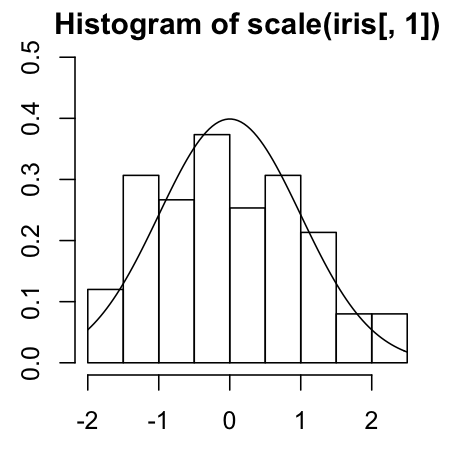
\includegraphics{figure/md-docx-fig1.png}
\caption{ヒストグラム}
\end{figure}

\end{block}

\end{frame}

\begin{frame}{最後に}

Enjoy!!

\end{frame}
